\section{Principal Component Analysis}
%\fixme{The amount of variation explained as a function of the number of PCA com- ponents included}
%\fixme{the principal directions of the considered PCA components}
%\fixme{the data projected onto the considered principal components}

In Principal Component Analysis the goal is to represent $N$-dimensional data using less then N numbers. This is done by finding $M$ orthogonal directions in which the data have the most variance and ignore the directions in where the data do not variance much. These $M$ principal directions form a lower-dimensional subspace and a $N$-dimensional data point can be represented by its projections onto these $M$ directions in the lower dimension subspace. The information about where the data is located in the remaining $N-M$ orthogonal directions are therefore lost. Since these do not have much variance, only a little information is lost.

\begin{figure}[H]
\centering
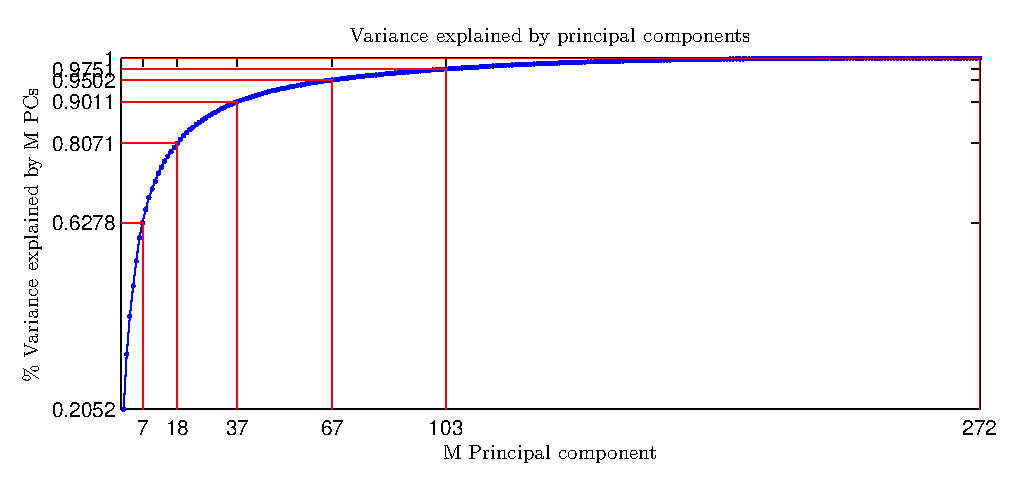
\includegraphics[width=\linewidth]{var_explained}
\caption{The variance explained by $M$ Components.\label{fig:pca_var_explained}}
\end{figure}

\subsection{Percent Variance Explained by $M$ Components}

In Figure~\ref{fig:pca_var_explained} the variance explained by $1$ to $M$ principal components are shown where the explained percent for one component are shown as around 19 percent. Then the components needed to explain 60, 80, 90, 96, 97 and 100 percent are marked out on the x axis respective to the percent explained variance on the y axis.

\subsection{Principal Components Directions}
Showing the PCs directions have not been dealt with in this report. We argue that it does not make much sense to show the directions from the original high dimensional data set as each attribute does not have any exact meaning. A better example for such is when we have a data set of attributes with exact meanings like workload and salary. Then a principal component could be directed to watch the two dimensions indicating that people who work hard make more money.


\subsection{Principal Component Projections}
By projecting the data onto the principal components we can by hand separate the classes based on the projections. Our hypothesis is then, that there exist a combination of PCs that will separate most classes. This is to be shown in the next assignments when we learn about classification.

\begin{figure}[H]
\centering
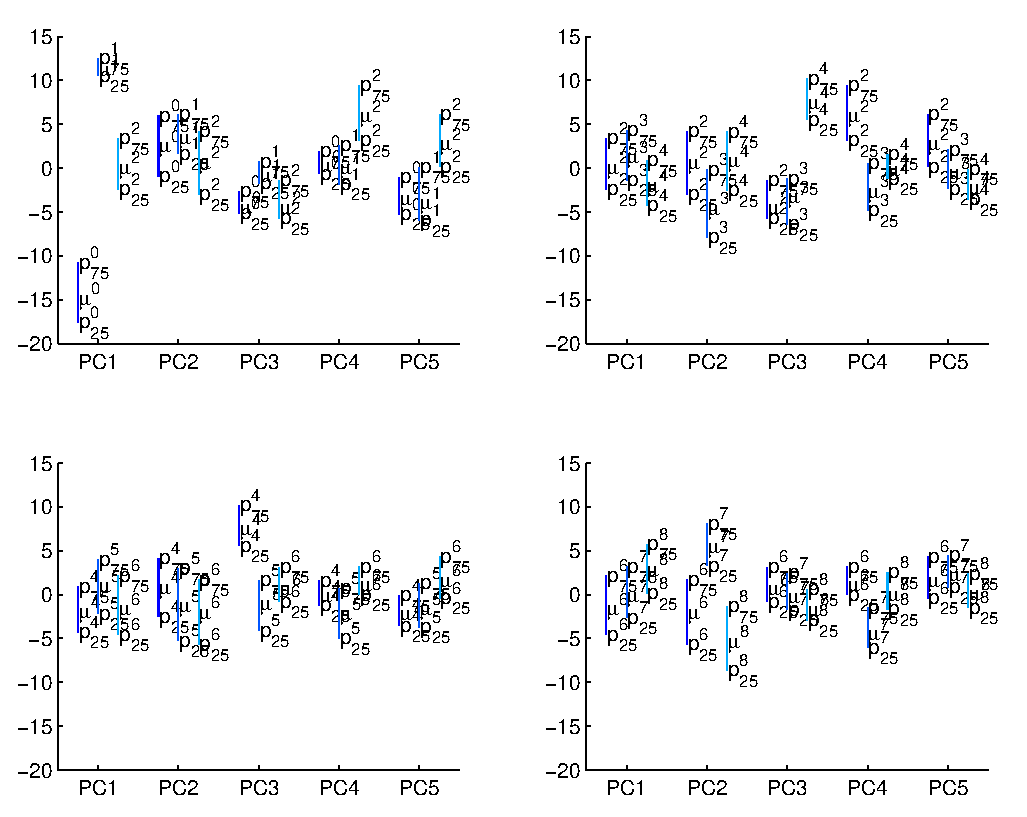
\includegraphics[width=\linewidth]{pca_projections_explained}
\caption{Here is nine of the ten classes shown as projections onto the principal components. Data are shown as median $\mu^{class}$ and $x={25,75}$ percentiles as $p_{x}^{class}$ for the first five components. For each PC three projections distributions are shown in each subplot. \label{fig:pca_projections_explained}}
\end{figure}

In Figure~\ref{fig:pca_projections_explained} it shows that the first PC are able to distinct class ${0,1}$ from each other along with all the other classes. PC three can distinct digit four. PC four can find digits of twos and sevens can be found using PC two. These are some examples that can be verified by human inspection. To classify further digits a linear combination of the projections will be needed and this is the real classification task if PCs was used as features. The problem is the same for our original features, its just not that trivial to separate them by hand as it was done here. Remembering how PCA have created linear combinations of the features such the most variance are in the first PC. 
